\documentclass{standalone}
\usepackage{tikz}
\usetikzlibrary{patterns, positioning}

\begin{document}
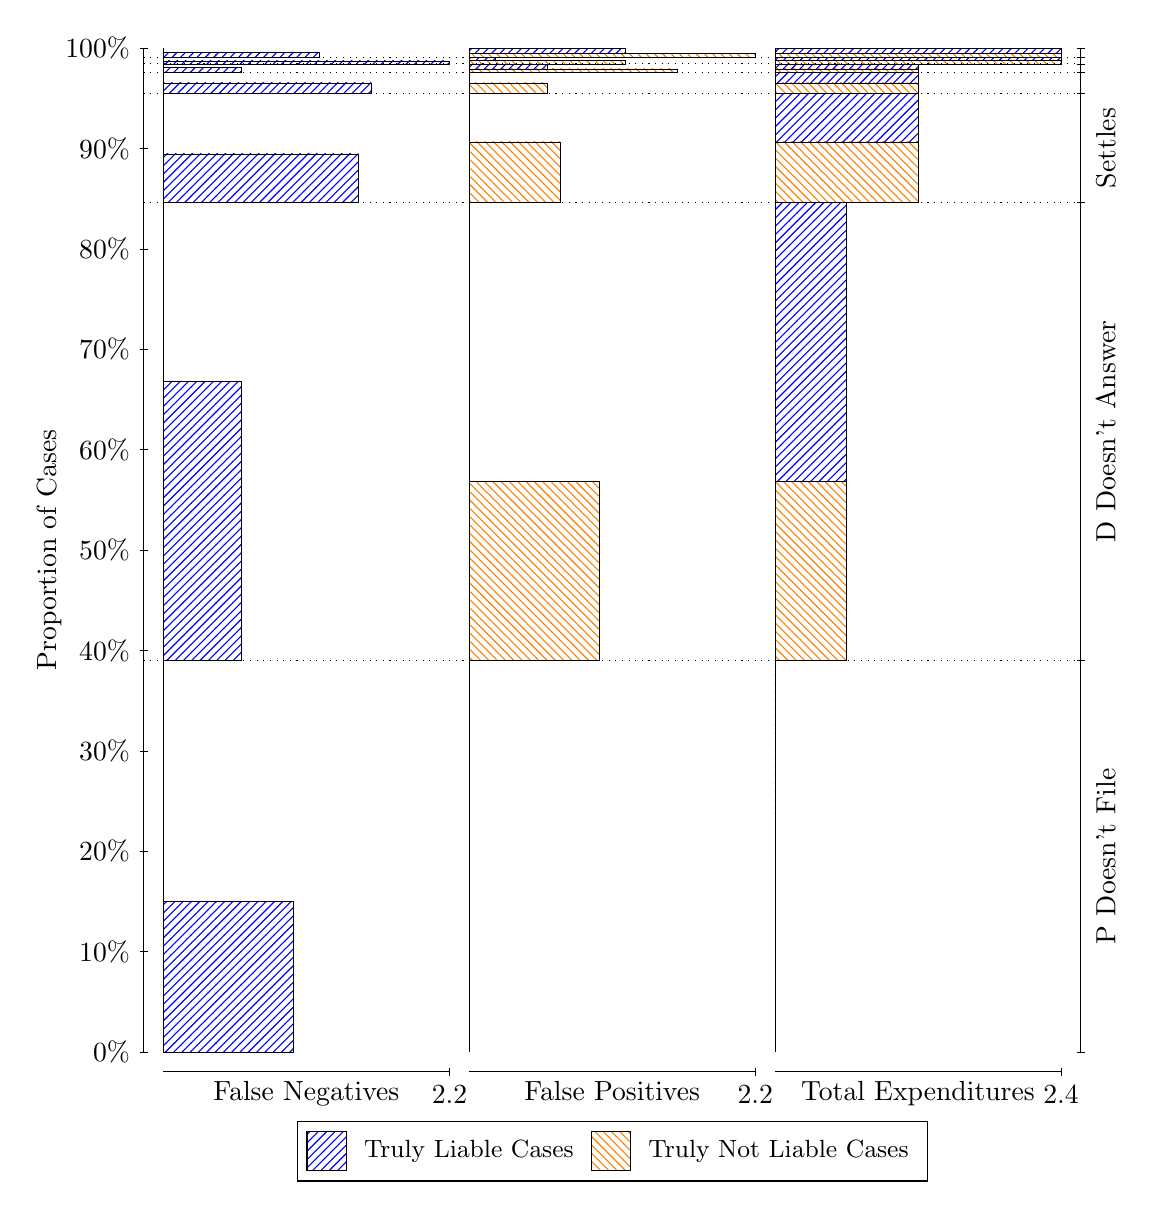
\begin{tikzpicture}
\draw[black, very thin] (1.5,1.75) -- (1.5,14.5);
\node[rotate=90, anchor=center] at (0.3, 8.125) {Proportion of Cases};
\draw[black, very thin] (1.45,1.75) -- (1.55,1.75);
\node[anchor=east] at (1.45, 1.75) {0\%};
\draw[black, very thin] (1.45,3.025) -- (1.55,3.025);
\node[anchor=east] at (1.45, 3.025) {10\%};
\draw[black, very thin] (1.45,4.3) -- (1.55,4.3);
\node[anchor=east] at (1.45, 4.3) {20\%};
\draw[black, very thin] (1.45,5.575) -- (1.55,5.575);
\node[anchor=east] at (1.45, 5.575) {30\%};
\draw[black, very thin] (1.45,6.85) -- (1.55,6.85);
\node[anchor=east] at (1.45, 6.85) {40\%};
\draw[black, very thin] (1.45,8.125) -- (1.55,8.125);
\node[anchor=east] at (1.45, 8.125) {50\%};
\draw[black, very thin] (1.45,9.4) -- (1.55,9.4);
\node[anchor=east] at (1.45, 9.4) {60\%};
\draw[black, very thin] (1.45,10.675) -- (1.55,10.675);
\node[anchor=east] at (1.45, 10.675) {70\%};
\draw[black, very thin] (1.45,11.95) -- (1.55,11.95);
\node[anchor=east] at (1.45, 11.95) {80\%};
\draw[black, very thin] (1.45,13.225) -- (1.55,13.225);
\node[anchor=east] at (1.45, 13.225) {90\%};
\draw[black, very thin] (1.45,14.5) -- (1.55,14.5);
\node[anchor=east] at (1.45, 14.5) {100\%};

\draw[black, very thin] (13.4,1.75) -- (13.4,14.5);
\draw[black, very thin] (13.35,1.75) -- (13.45,1.75);
\node[anchor=west] at (13.35, 1.75) {};
\draw[black, very thin] (13.35,6.7219) -- (13.45,6.7219);
\node[anchor=west] at (13.35, 6.7219) {};
\draw[black, very thin] (13.35,12.539) -- (13.45,12.539);
\node[anchor=west] at (13.35, 12.539) {};
\draw[black, very thin] (13.35,13.923) -- (13.45,13.923);
\node[anchor=west] at (13.35, 13.923) {};
\draw[black, very thin] (13.35,14.191) -- (13.45,14.191);
\node[anchor=west] at (13.35, 14.191) {};
\draw[black, very thin] (13.35,14.298) -- (13.45,14.298);
\node[anchor=west] at (13.35, 14.298) {};
\draw[black, very thin] (13.35,14.377) -- (13.45,14.377);
\node[anchor=west] at (13.35, 14.377) {};
\draw[black, very thin] (13.35,14.5) -- (13.45,14.5);
\node[anchor=west] at (13.35, 14.5) {};

\draw[black, very thin, pattern color=blue, pattern=north east lines] (1.75,1.75) rectangle (3.4015,3.6597);
\draw[black, very thin, pattern color=orange, pattern=north west lines] (1.75,3.6597) rectangle (1.75,6.7219);
\draw[black, very thin, pattern color=blue, pattern=north east lines] (1.75,6.7219) rectangle (2.7409,10.266);
\draw[black, very thin, pattern color=orange, pattern=north west lines] (1.75,10.266) rectangle (1.75,12.539);
\draw[black, very thin, pattern color=blue, pattern=north east lines] (1.75,12.539) rectangle (4.2273,13.155);
\draw[black, very thin, pattern color=orange, pattern=north west lines] (1.75,13.155) rectangle (1.75,13.923);
\draw[black, very thin, pattern color=blue, pattern=north east lines] (1.75,13.923) rectangle (4.3924,14.056);
\draw[black, very thin, pattern color=orange, pattern=north west lines] (1.75,14.056) rectangle (1.75,14.191);
\draw[black, very thin, pattern color=blue, pattern=north east lines] (1.75,14.191) rectangle (2.7409,14.254);
\draw[black, very thin, pattern color=orange, pattern=north west lines] (1.75,14.254) rectangle (1.75,14.298);
\draw[black, very thin, pattern color=blue, pattern=north east lines] (1.75,14.298) rectangle (5.3833,14.336);
\draw[black, very thin, pattern color=orange, pattern=north west lines] (1.75,14.336) rectangle (1.75,14.377);
\draw[black, very thin, pattern color=blue, pattern=north east lines] (1.75,14.377) rectangle (3.7318,14.447);
\draw[black, very thin, pattern color=orange, pattern=north west lines] (1.75,14.447) rectangle (1.75,14.5);
\draw[black, very thin, pattern color=orange, pattern=north west lines] (5.6333,1.75) rectangle (5.6333,4.8121);
\draw[black, very thin, pattern color=blue, pattern=north east lines] (5.6333,4.8121) rectangle (5.6333,6.7219);
\draw[black, very thin, pattern color=orange, pattern=north west lines] (5.6333,6.7219) rectangle (7.2848,8.995);
\draw[black, very thin, pattern color=blue, pattern=north east lines] (5.6333,8.995) rectangle (5.6333,12.539);
\draw[black, very thin, pattern color=orange, pattern=north west lines] (5.6333,12.539) rectangle (6.7894,13.307);
\draw[black, very thin, pattern color=blue, pattern=north east lines] (5.6333,13.307) rectangle (5.6333,13.923);
\draw[black, very thin, pattern color=orange, pattern=north west lines] (5.6333,13.923) rectangle (6.6242,14.057);
\draw[black, very thin, pattern color=blue, pattern=north east lines] (5.6333,14.057) rectangle (5.6333,14.191);
\draw[black, very thin, pattern color=orange, pattern=north west lines] (5.6333,14.191) rectangle (8.2758,14.235);
\draw[black, very thin, pattern color=blue, pattern=north east lines] (5.6333,14.235) rectangle (6.6242,14.298);
\draw[black, very thin, pattern color=orange, pattern=north west lines] (5.6333,14.298) rectangle (7.6152,14.339);
\draw[black, very thin, pattern color=blue, pattern=north east lines] (5.6333,14.339) rectangle (5.9636,14.377);
\draw[black, very thin, pattern color=orange, pattern=north west lines] (5.6333,14.377) rectangle (9.2667,14.429);
\draw[black, very thin, pattern color=blue, pattern=north east lines] (5.6333,14.429) rectangle (7.6152,14.5);
\draw[black, very thin, pattern color=orange, pattern=north west lines] (9.5167,1.75) rectangle (9.5167,4.8121);
\draw[black, very thin, pattern color=blue, pattern=north east lines] (9.5167,4.8121) rectangle (9.5167,6.7219);
\draw[black, very thin, pattern color=orange, pattern=north west lines] (9.5167,6.7219) rectangle (10.425,8.995);
\draw[black, very thin, pattern color=blue, pattern=north east lines] (9.5167,8.995) rectangle (10.425,12.539);
\draw[black, very thin, pattern color=orange, pattern=north west lines] (9.5167,12.539) rectangle (11.333,13.307);
\draw[black, very thin, pattern color=blue, pattern=north east lines] (9.5167,13.307) rectangle (11.333,13.923);
\draw[black, very thin, pattern color=orange, pattern=north west lines] (9.5167,13.923) rectangle (11.333,14.057);
\draw[black, very thin, pattern color=blue, pattern=north east lines] (9.5167,14.057) rectangle (11.333,14.191);
\draw[black, very thin, pattern color=orange, pattern=north west lines] (9.5167,14.191) rectangle (11.333,14.235);
\draw[black, very thin, pattern color=blue, pattern=north east lines] (9.5167,14.235) rectangle (11.333,14.298);
\draw[black, very thin, pattern color=orange, pattern=north west lines] (9.5167,14.298) rectangle (13.15,14.339);
\draw[black, very thin, pattern color=blue, pattern=north east lines] (9.5167,14.339) rectangle (13.15,14.377);
\draw[black, very thin, pattern color=orange, pattern=north west lines] (9.5167,14.377) rectangle (13.15,14.429);
\draw[black, very thin, pattern color=blue, pattern=north east lines] (9.5167,14.429) rectangle (13.15,14.5);
\draw[black, dotted] (1.5,6.7219) -- (13.4,6.7219);
\draw[black, dotted] (1.5,12.539) -- (13.4,12.539);
\draw[black, dotted] (1.5,13.923) -- (13.4,13.923);
\draw[black, dotted] (1.5,14.191) -- (13.4,14.191);
\draw[black, dotted] (1.5,14.298) -- (13.4,14.298);
\draw[black, dotted] (1.5,14.377) -- (13.4,14.377);
\draw[black, very thin] (1.75,1.5) -- (5.3833,1.5);
\node[anchor=north] at (3.5667, 1.5) {False Negatives};
\draw[black, very thin] (5.3833,1.45) -- (5.3833,1.55);
\node[anchor=north] at (5.3833, 1.45) {2.2};

\draw[black, very thin] (5.6333,1.5) -- (9.2667,1.5);
\node[anchor=north] at (7.45, 1.5) {False Positives};
\draw[black, very thin] (9.2667,1.45) -- (9.2667,1.55);
\node[anchor=north] at (9.2667, 1.45) {2.2};

\draw[black, very thin] (9.5167,1.5) -- (13.15,1.5);
\node[anchor=north] at (11.333, 1.5) {Total Expenditures};
\draw[black, very thin] (13.15,1.45) -- (13.15,1.55);
\node[anchor=north] at (13.15, 1.45) {2.4};

\node[black, centered, rotate=90] at (13.72, 4.2359) {P Doesn't File};
\node[black, centered, rotate=90] at (13.72, 9.6307) {D Doesn't Answer};
\node[black, centered, rotate=90] at (13.72, 13.231) {Settles};





\draw (7.449999999999999,1.5) node[draw=none] (baseCoordinate) {};
\begin{scope}[align=center]
        \matrix[scale=0.5, draw=black, below=0.5cm of baseCoordinate, nodes={draw}, column sep=0.1cm]{
            \node[rectangle, draw, minimum width=0.5cm, minimum height=0.5cm, pattern=north east lines, pattern color=blue] {}; &
            \node[draw=none, font=\small] (B) {Truly Liable Cases}; &
            \node[rectangle, draw, minimum width=0.5cm, minimum height=0.5cm, pattern=north west lines, pattern color=orange] {}; &
            \node[draw=none, font=\small] (B) {Truly Not Liable Cases}; \\
            };
\end{scope}

\end{tikzpicture}
\end{document}